% !TEX root = ../main.tex
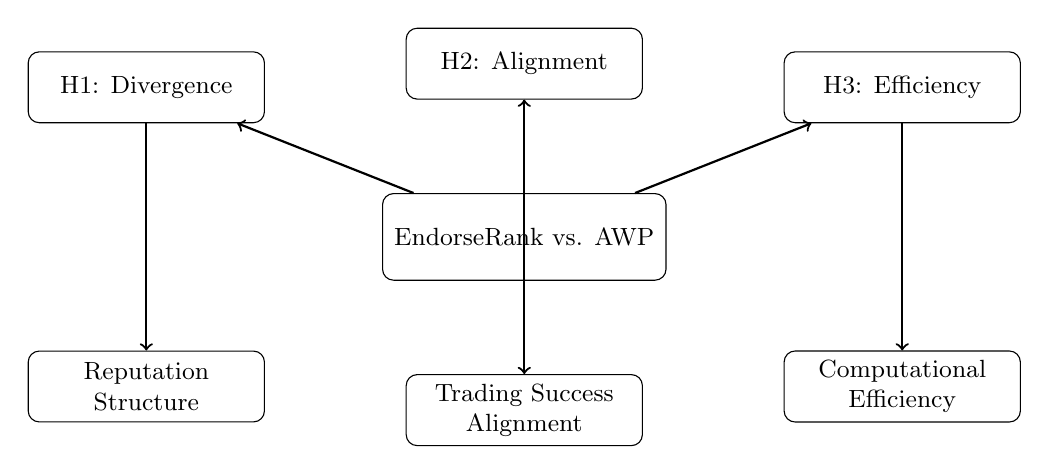
\begin{tikzpicture}[
  font=\small,
  box/.style={draw, rounded corners, align=center, minimum width=3.6cm, minimum height=1.1cm},
  smallbox/.style={draw, rounded corners, align=center, minimum width=3.0cm, minimum height=0.9cm},
  arrow/.style={->, thick}
]
\node[box] (center) at (0,0) {EndorseRank vs. AWP};
\node[smallbox] (h1) at (-4.8,1.9) {H1: Divergence};
\node[smallbox] (rep) at (-4.8,-1.9) {Reputation\\Structure};
\node[smallbox] (h2) at (0,2.2) {H2: Alignment};
\node[smallbox] (risk) at (0,-2.2) {Trading Success\\Alignment};
\node[smallbox] (h3) at (4.8,1.9) {H3: Efficiency};
\node[smallbox] (eff) at (4.8,-1.9) {Computational\\Efficiency};
\draw[arrow] (center) -- (h1);
\draw[arrow] (center) -- (h2);
\draw[arrow] (center) -- (h3);
\draw[arrow] (h1) -- (rep);
\draw[arrow] (h2) -- (risk);
\draw[arrow] (h3) -- (eff);
\end{tikzpicture}
